\documentclass[a4paper,11pt]{jsarticle} % ceostyを用いるための文書クラス

% 冊子形式にするには表紙(ページ数に含まれない)で
% 1ページ使っているので最後のページのページ番号が
% 4n  ->透かしがしにくい(表紙と裏表紙の裏面が白紙)
% 4n+1->一番微妙
% 4n+2->表紙と白紙の裏表紙ができる---こうなるように調整
% 4n+3->裏表紙も使う

\usepackage{fancyhdr}	% ページスタイル

%%スタイル
% 数式やテキストの描画
\usepackage{amsmath, amsfonts, amssymb, mathtools, mathrsfs, latexsym}	% ams関連は数式書くのに必須!!
%\DeclarePairedDelimiter{\abs}{\lvert}{\rvert}
\usepackage{nccmath, empheq}	% 結構ピンポイントなパッケージ

% 画像
%% 枠だけ表示(Cannot determine size of graphicと結構怒られる)
%\usepackage[draft]{graphicx}
%% 普通に表示させる(ただ重くなりやすい)
\usepackage[dvipdfmx]{graphicx}
\usepackage[dvipdfmx]{color}
\usepackage{here}	% 絶対Hereって勝手に呼んでるやつ
\usepackage{wrapfig}	% 回り込み(ceostyのymawarikomiもある)
\usepackage{subcaption}	% minipageを使って図を並べるときの各画像のキャプションに必要

% このファイルの肝.
% usepackageの順番(ceoとの前後関係)を変えると途端にエラーを吐くので注意
%\usepackage{ceo}
% 以下のパッケージはceostyの煽りをくらったもの
\usepackage{enumerate, comment}	% 順に文書モードでの段落環境, 複数行コメント

\pagestyle{fancy}
  \lhead{2023年10月21日}
  \rhead{第1問}
  \cfoot{\thepage}

\newcommand{\vevenspace}{\vspace{\stretch{1}}}	
\newcommand{\hruleline}{\par\noindent\hrulefill\par}
\newcommand{\length}[1]{$\overline{\textup{#1}}$}
\renewcommand{\eq}{$=$}
\newcommand{\vreidai}{\vspace{\stretch{0.3}}}
\newcommand{\nn}{$n$}
\newcommand{\m}{$m$}
\newcommand{\kmath}{$k$}
\renewcommand{\O}{\textup{O}}
\newcommand{\Pn}[2]{$\textup{#1}_{#2}$}
\newcommand{\mathPn}[2]{\textup{#1}_{#2}}
\renewcommand{\P}{\textup{P}}
\newcommand{\Q}{\textup{Q}}
\newcommand{\R}{\textup{R}}
\newcommand{\A}{\textup{A}}
\newcommand{\B}{\textup{B}}
\newcommand{\C}{\textup{C}}
\newcommand{\D}{\textup{D}}
\newcommand{\numseq}[2]{$\{#1_{#2}\}$}
\newcommand{\combi}[2]{{}_{#1}\mathrm{C}_{#2}}
\newcommand{\xy}{$xy$}
\newcommand{\yz}{$yz$}
\newcommand{\xz}{$xz$}
\newcommand{\zx}{$zx$}
\newcommand{\xyz}{$xyz$}
\newcommand{\x}{$x$}
\newcommand{\y}{$y$}
\newcommand{\z}{$z$}
\newcommand{\g}{$g$}

\newcounter{numEq}
\newcommand{\assignNumEq}{%
\stepcounter{numEq}
\tag*{$\cdots\cdots$\ctext{\the\value{numEq}}}
}
\newcommand{\ctext}[1]{\raise0.2ex\hbox{\textcircled{\scriptsize{#1}}}}

%%%%%%%%%% メイン %%%%%%%%%%%
\begin{document}
%!TEX root = *.tex
%%%%%%%%%%%%%%%%%%
% カウンタのリセット
% 問題文
滑車と糸の質量は無視できるものとし,重力加速度を\g とする.

\begin{enumerate}[〔A〕]
  \setlength{\leftskip}{-1.5zw}
  \setlength{\itemindent}{1zw}\setlength{\labelsep}{0.5zw}
  \setlength{\labelwidth}{1zw}\setlength{\leftmargin}{1zw}
  \setlength{\itemsep}{0.5\baselineskip}
  \item 図1のように,なめらかに回る定滑車に伸縮しない糸をかけて,糸の一方に質量$m_1$のおもりA,他方に質量$m_2$のおもりBをつけて静かに放した.
  \begin{enumerate}[(1)]
    \setlength{\leftskip}{-2.5zw}
    \setlength{\itemindent}{1zw}\setlength{\labelsep}{1zw}
    \setlength{\labelwidth}{1zw}
    \item $m_1 > m_2$のとき,おもりAが下降する加速度の大きさを求めよ.
    \item 糸に働く張力の大きさを求めよ.
    \item $m_1 + m_2 = \text{一定}$として,糸の張力を最大にする$m_1$と$m_2$の関係を求めよ.
  \end{enumerate}
  \item 次に,図2のように定滑車の一方に質量$3M$のおもりCを,他方に動滑車をつり下げて,動滑車には質量$2M$のおもりDと質量$M$のおもりEをつり下げた.C,D,Eを同時に静かに放した.
  \begin{enumerate}[(1)]
    \setlength{\leftskip}{-2.5zw}
    \setlength{\itemindent}{1zw}\setlength{\labelsep}{1zw}
    \setlength{\labelwidth}{1zw}
    \item おもりC,D,Eの加速度の大きさを求めよ.
    \item おもりD,E間の糸に働く張力の大きさを求めよ.
    \item おもりD,EはそのままでおもりCを$\C^\prime$に換えると,$\C^\prime$,D,Eを同時に静かに放しても,おもりは静止したまま動かなかった.
    このときのおもり$\C^\prime$の質量を求めよ.
  \end{enumerate}
\end{enumerate}

\begin{figure}[htbp]
  \centering
  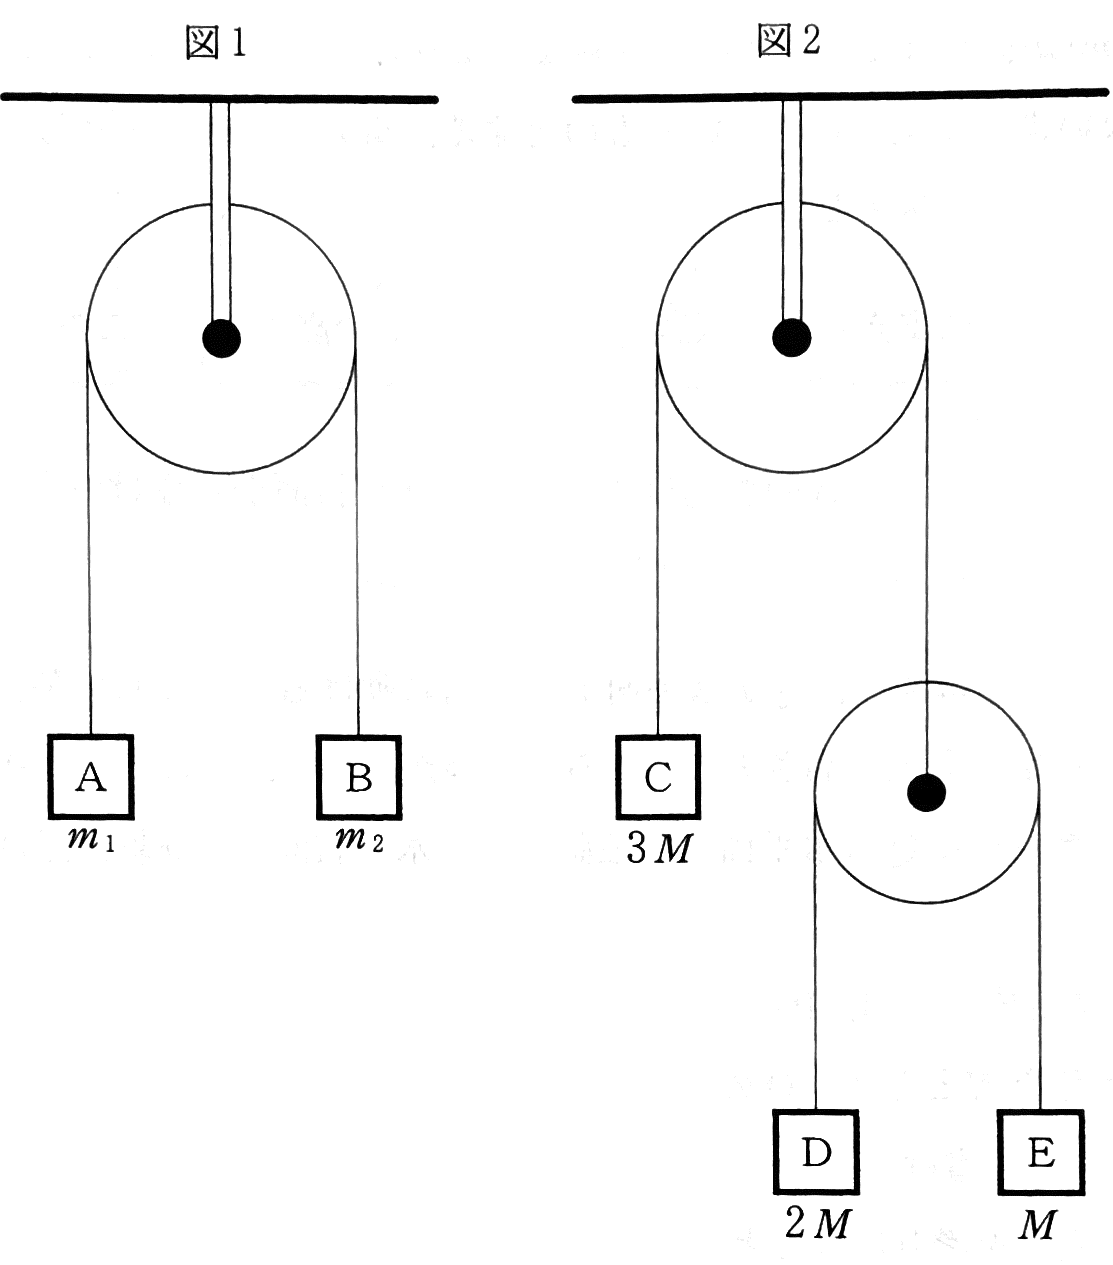
\includegraphics[width=20zw]{../graphs/se_1H_102.png}
\end{figure}


% メモ
\begin{comment}

\end{comment}


%%%%%%%%%%%%%%%%%%

\hruleline
%!TEX root = *.tex
%%%%%%%%%%%%%%%%%%
% メモ
\begin{comment}

\end{comment}
% カウンタのリセット
\setcounter{eqNo}{0}
% 解答
\noindent {\large【解答】\par}

\noindent 〔A〕\par 
\noindent \,(1)\,
$T$を糸の張力とし,$a$をおもりAが下降する加速する加速度の大きさとする.
おもりA,Bについて運動方程式
\begin{align*}
  m_1 a = m_1 g -T \assignEqNo\\
  m_2 a = T - m_2 g \assignEqNo
\end{align*}
\ctext{1},\ctext{2}より
\begin{align*}
  (m_1 + m_2)a &= (m_1 - m_2)g\\
  a &= \dfrac{m_1-m_2}{m_1+m_2}g
\end{align*}

\noindent \,(2)\,
\ctext{1}と(1)の結果から,
\begin{align*}
  T = \dfrac{2m_1m_2}{n_1+m_2}g
\end{align*}
である.

\noindent \,(3)\,
$m_1=m_2=m$(定数)とおく.このとき,(2)の結果から,
\begin{align*}
  T = \dfrac{2m_1(m-m_1)}{m_1+m_2}g
\end{align*}
となる.これより,$T$は$m_1=\dfrac{m}{2}$のとき最大である.すなわち,
$m_1=m_2$.

\noindent 〔B〕\par 
\noindent\,(4)
$C$が糸からうける張力を$T_1$,Dが糸からうける張力を$T_2$とする.
また,$\alpha,\,\beta,\,\gamma$をそれぞれ,C,D,Eの加速度とし,すべて鉛直下向きを正とする.
このとき,運動方程式
\begin{align*}
  3M \alpha &= 3Mg - T_1 \assignEqNo\\
  2M \beta &= 2Mg - T_2 \assignEqNo\\
  M \gamma &= Mg - T_3 \assignEqNo
\end{align*}
加えて動滑車は糸を介しておもりCとつながっているので,加速度は$-\alpha$であり,運動方程式より
\begin{align*}
  0 = 2T_2 - T_1 \assignEqNo
\end{align*}
また,DとEも動滑車を間にして糸でつながっているので,動滑車に対する相対加速度の和はゼロベクトルとなるので,
\begin{align*}
  (\beta - (-\alpha)) + (\gamma - (-\alpha)) &= 0 \\
  \therefore 2\alpha + \beta + \gamma &= 0
\intertext{となり,両辺に$M$を乗じて}
  2M\alpha + M\beta + M\gamma &= 0 \assignEqNo
\end{align*}
を得る.
いま,\ctext{3},\ctext{4},\ctext{5}を\ctext{7}に代入して
\begin{align*}
  &2(Mg-\dfrac{1}{3}T_1) + (Mg - \dfrac{1}{2}T_2) + (Mg-T_2) = 0\\
  &\ \therefore 4T_1 + 9T_2 = 24Mg \assignEqNo
\end{align*}
\ctext{6},\ctext{8}を連立して解くと
\begin{align*}
  T_1 = \dfrac{48}{17}Mg,\quad T_2 = \dfrac{24}{17}Mg
\end{align*}
であり,\ctext{3},\ctext{4},\ctext{5}より
\begin{align*}
  \alpha = \dfrac{1}{17}g,\ \beta = \dfrac{5}{17}g,\ \gamma = -\dfrac{7}{17}g
\end{align*}
以上より,C,D,Eの加速度の大きさはそれぞれ
$\dfrac{1}{17}g,\,\dfrac{5}{17}g,\,\dfrac{7}{17}g$.

\noindent \,(5)\, (4)の過程より$T_2=\dfrac{24}{17}Mg$.

\noindent \,(6)\, Cが静止しているということは,動滑車も静止している.
すなわち,定滑車とみなすことができる.
よって,D,Eの運動は〔A〕で$m_1=2M,\,m_2=M$としたときの運動に一致する.
したがってDがうける張力の大きさ$S_2$は
\begin{align*}
  S_2 = \dfrac{2m_1m_2}{m_1+m_2}g = \dfrac{4}{3}Mg
\end{align*}
さらに,動滑車にはたらく力のつりあいより,$\C^\prime$がうける張力の大きさは$\dfrac{8}{3}Mg$である.よって,$\C^\prime$の運動方程式より
\begin{align*}
  M^\prime\cdot 0 &= M^\prime g - \dfrac{8}{3}Mg \\
  \therefore M^\prime &= \dfrac{8}{3}M 
\end{align*}

%%%%%%%%%%%%%%%%%%

\end{document}